% class options:
% - select either [german] or [english]
% - select the type of thesis from:
%   [bachelor, master, generic]
%   (in case of generic, use \type{} to specify it)
% - use option "alpha" for abbreviated citation (instead of numbers)
% - option "draft" is available, too
% - use options "utf8" or "latin1" to select inputencoding
\documentclass[english, master, utf8]{base/thesis_KBS}

\usepackage{units}    % useful for settings units:              \unit[23]{m}
\usepackage{nicefrac} % for setting fractions esp. within text: \nicefrac{km}{h}

\usepackage{algorithm, algorithmic}  % for pseudo code (cf. documentation)
\renewcommand{\algorithmiccomment}[1]{\qquad{\small // \textit{#1}}}

% for code keywords within the text
\usepackage{xcolor}
\definecolor{light-gray}{gray}{0.95}
\newcommand{\code}[1]{\colorbox{light-gray}{\texttt{#1}}}

%%%%%%%%%%%%%%%%%%%%%%%%%%%%%%%%%%%%%%%%%%%%%%%%%%%%%%%%%%%%%%%%%%%%%%%%%%%%%%%

\begin{document}

\title{Execution Monitoring for Long-Term Autonomous Plant Observation with a Mobile Robot}
\author{Tim Bohne}
\email{tbohne@uni-osnabrueck.de}
\firstSupervisor{Prof. Dr. Joachim Hertzberg}
\secondSupervisor{Benjamin Kisliuk, M.Sc.}
%\shorttitle{...}                       % by default = title
%\dept{...}                             % by default KBS UOS
%\submitdate{November 2004}             % by default current month & year
%\signcity{}                            % by default Osnabr�ck
%signline{Osnabr�ck, 11. Dezember 2004} % by default "signcity, submitdate"

\generatetitle

\cleardoublepage

\begin{prefacesection}{Abstract}
TBD. \dots
\end{prefacesection}

\cleardoublepage
\tableofcontents

\startTextChapters %%%%%%%%%%%%%%%%%%%%%%%%%%%%%%

\chapter{Introduction}

ADD INTRO TEXT: Why is LTA interesting and relevant for agriculture?\newline

As the title suggests, the goal of this work is to integrate a prototypical system for long-term autonomous plant observation that is able to address 
particular challenges for long-term autonomy in such a context through the use of execution monitoring methods. Initially, typical challenges that may stand in the way of a mobile
robot's long-term autonomy in an agricultural setting will be identified. Afterwards, a subset of these challenges will be studied systematically in order to 
approach robust solutions. Accordingly, the prolonged objective is to increase the number of situations in which a mobile robot is able to 
overcome such challenges by itself. However, the mere recognition of problematic situations is already of decisive advantage from a practical perspective,
as the robot is then able to communicate the problem and request help, e.g. from a human operator, instead of undeliberately aborting its mission.
In addition, a prerequisite for solving a problem is, of course, recognizing it. Therefore, a major aim of this work is to develop execution monitoring
approaches that enable the robot to detect unexpected problematic situations that require special treatment.\newline

\textbf{Expected Scientific Contribution}\newline

Key challenges that may prevent long-term autonomous mobile robots in a field monitoring context from working properly will be identified, implemented 
in a simulation and systematically evaluated. A major objective of this work is to address a subset of these challenges based on execution monitoring approaches,
i.e. to propose methods that are capable of partially resolving or at least detecting such issues in order to enable the robot to communicate them to a human operator,
e.g. by a push message to the phone. The mere recognition of such situations would already be a decisive advantage from a practical perspective. Moreover, if it is possible
to show that with the solutions developed in this work the number of failures can be reduced by a certain percentage, distributed over a fraction of cases in which the robot 
recognizes a problem and calls the operator for help, and a fraction in which it is even able to solve the problem itself, the system can be considered a relevant step towards 
the overall goal of robust, long-term autonomous field monitoring robots. In other words, it is a suitable performance criterion that allows an empirical analysis to
determine whether the proposed methods are indeed able to improve the robustness of the system. In summary, this work attempts to reduce the barriers towards long-term
autonomy of mobile field monitoring robots by demonstrating a fully integrated solution capable of addressing some of the typical problems for such systems.\newline

\textbf{Approach}\newline

The idea is to start with the basic long-term autonomy setup described in section \ref{sec:scientific_bg}, provide a list of potential problems that 
stand in its way, and develop execution monitoring methods to detect a subset of these issues with the aim of increasing the robustness of such a system in a simulation
and ideally in practice on the real hardware. In the end, there should be a working system that addresses some of the problems of long-term autonomy 
in scenarios similar to the one described in section \ref{sec:lta_plant_observation}. The nature of the work is going to be integrative and application-oriented. The modules 
needed to set up the initial prototype are available in principle, but it will be part of this work to integrate and extend them in order to end up with a holistic and robust
solution. After the basic scenario works in the simulation, it is going to be extended with an evaluation part. A subset of the potential barriers described in section 
\ref{sec:challenges_for_lta} is going to be implemented and it will be shown that the system no longer works under certain conditions, i.e. that these
barriers are indeed able to cause failure of long-term autonomous systems. Consequently, a first step is to observe how the system performs without any further 
treatment of such problematic situations, i.e. how often the robot gets stuck in the simulation based on a specific problem case.
Subsequently, the goal is to develop monitoring methods capable of recognizing these problems such that they can be resolved.
To give an example, a particular idea could be to block paths on the field in the simulation in a randomized fashion with the intent of reproducibly making things that 
can go wrong actually go wrong. The type of the obstacles is incidental to this work, e.g. a muddy path that the robot is not able to drive through. 
It is obvious that the robot must be enabled to detect such problems, in this case by some kind of obstacle detection.
Once detected, the problem can be resolved by either incorporating solutions from the literature or finding new solutions.
Since detection is a necessary prerequisite for overcoming these barriers, the focus will be on detection, i.e. execution monitoring,
and an initial trivial solution adopted for all of them is to call the human operator who then takes care of the problem.\newline
As should be clear by now, long-term autonomy, as robotics in general, is an integration problem. Many technologies have to be integrated in order to build a working system, 
and compared to other disciplines of artificial intelligence, it is not trivial to evaluate the system and conclude, for example, that it has improved the status quo by a 
certain percentage. Nevertheless, it is crucial to provide results that are meaningful based on scientific standards. 
The keyword under which such attempts are summarized is scientific robotics, and a goal of this work will be to evaluate the developed system based on these standards.
Since it is beyond the scope of this work to test the developed system for extended periods of time in practice, there is a need for other ways of evaluation.
This is where the described evaluation approach in the simulation comes into play. In order to demonstrate, test and evaluate the system, there will be a sufficiently meaningful, 
i.e. realistic, physics simulation that allows an empirical analysis based on a huge number of samples. As mentioned, the starting point will be the simulation from the 
PORTAL project that is going to be extended as part of this work. Ultimately, there should also be a long-term test (e.g. one day) in the field with the real hardware that 
underlines the relevance of the approaches discussed in this work for practical applications. However, since a mobile robot is a complex system, there are arbitrary 
many technical barriers that could prevent such a long-term test in the real world. The idea is therefore to be at least able to demonstrate the system in the simulation
without depending on the success of such a real-world experiment. In addition to serving as a backup for possible failures in real-world tests,
a simulation naturally creates an environment that allows reproducible situations and thus permits empirical investigation.

ADD CHAPTER OVERVIEW \dots\newline

\chapter{Long-Term Autonomous Mobile Robots}

Long-term autonomous mobile robotic systems can be of great benefit in diverse environments. For the most part, in activities that are either too dangerous,
or too undemanding (e.g. monotonous, not meaningful) to be performed by humans. In addition, economic considerations can play a role, as well as tasks 
that are undesirable for other reasons, e.g. because they are considered dirty.
All three attributes - \textit{long-term}, \textit{autonomous}, and \textit{mobile} - have the potential of dramatically increasing the complexity and
the risk for failures of the system. Part of this chapter will be to precisely define what each of the attributes means in the context of this work.
The attribute of mobility is the easiest to define: A mobile robot is a system capable of moving freely (within limits) through an environment. \cite{Hertzberg:2012}
Thus, it's about the ability of a robot to move rather than being statically attached to a position.
Section \ref{sec:lta_plant_observation} introduces the scenario that is going to be studied in this work and provides a definition for the concept of long-term 
autonomy as understood in the following chapters, i.e. clarifies what the two remaining attributes \textit{long-term} and \textit{autonomous} are supposed to mean.
Afterwards, in section \ref{sec:scientific_bg}, the scientific and technological background that forms the basis of this work is discussed. 
Finally, section \ref{sec:challenges_for_lta} identifies potential hinderances for long-term autonomous systems with a particular focus on the considered plant monitoring scenario.

\section{Long-Term Autonomous Plant Observation}
\label{sec:lta_plant_observation}

The particular scenario that is going to be considered in this work takes place in an agricultural context.
The idea is to enable a mobile robot to autonomously conduct 3D-Lidar scans and hyperspectral images of the plants on a field in order to monitor their growth progression and 
to detect certain features based on the growth stage. Moreover, these recordings can be used to detect leaf diseases [TODO: refine based on literature].
Correspondingly, the robot has to be able to process the entire field continually without the need for human supervision,
including the requirement for repeated charge stops. For this purpose, there is supporting infrastructure in the form of a container with an inductive charging station on site
establishing the power supply. Since the focus of the work is not going to be the scanning task, but to establish robust long-term autonomy, the actual detection of features 
etc. will be disregarded.
A crucial question is how to actually define ``long-term''. As Hawes et al. remark, it has no strict definition and can have various meanings depending
on the context, e.g. NASA's rover \textit{Opportunity} has been exploring the surface of Mars autonomously for years and autonomous wave gliders are able to monitor
ocean sections for months. Furthermore, there are mobile service robots used for extended periods of time in everyday, indoor environments like hospitals 
as examined in the STRANDS project. \cite{Hawes:2017}
For this work, in contrast, ``long-term'' is going to be defined in terms of the robot's temporal radius of action that is mainly based on its battery capacity, i.e. charge cycle,
but may also include aspects like maintenance intervals etc. In general, all processes that require a number of such cycles are considered long-term processes.
Accordingly, ``long-term'' can only be defined depending on the system in question. To give an example: There are systems with very limited battery capacity, 
such as toy drones. Based on absolute time, a two-hour experiment might not be regarded as being long-term, but if it involves multiple charging cycles, it can be 
algorithmically considered a long-term process. Consequently, ``long-term'' is relative.\newline
In the agricultural sector, there are processes that last much longer than a charge cycle, e.g. vegetation periods.
However, the seasonal cycle is not the sort of long-term process that will be investigated in this work, as such processes already exist on a much smaller scale.
On the one hand, there is the mission level, i.e. one processing of an entire field. 
Such a mission can already be regarded as long-term, since based on the dimensions of the particular field under consideration, it is not guaranteed that one
battery charge will be sufficient to process the entire field. Instead, one battery cycle will be defined as sufficient to process a certain fraction of the scan
positions, and a planner should maximize the number of planned scan stops in a mission under the constraint that a battery safety buffer is not undercut.
Thus, a key aspect of the scenario is going to be that the mission must be paused, the state must be saved, and the mission must be continued after recharging.
In the meantime, the environment may have changed, e.g. weather conditions or illumination, which is relevant for certain sensors of the robot.
On the other hand, there are going to be several such field processings during one vegetation period, which makes it a long-term process of repeated missions.
Hence, it takes a number of charge cycles to process the entire field, and that mission is going to be repeated every few days,
which means that there are two different long-term cycles that are intertwined.
These two cycles basically represent a lower bound for the length of long-term autonomous episodes in the scenario under
consideration. Likewise, in contrast to the above examples of Mars rovers and autonomous wave gliders, which are long-term
processes of arbitrary length, it is useful to think about natural upper bounds on the length of such episodes in agricultural
applications. Such a natural upper bound could be a time after which a human operator will inspect the robot anyway,
which in agriculture is certainly the case sooner than after a few months, e.g. during maintenance sessions 
when sensors such as cameras and laser scanners are cleaned, tire pressures are checked, etc.
After such a maintenance session, the new episode begins. 
Based on these bounds, it makes sense that the robot does not send every minor problem it recognizes directly to the operator,
but keeps a list of minor issues that do not require immediate action, but should be resolved during the next maintenance
appointment.\newline
Now that it has been sufficiently clarified how \textit{long-term} and \textit{mobile} are to be understood in the context of this work,
a precise definition of what is meant by the remaining attribute \textit{autonomous} follows.
Like the concept \textit{long-term}, \textit{autonomous} is not sharply defined in the literature and can have different meaningful connotations depending
on the context. Autonomy in the context of application-oriented robots usually has the goal of achieving a higher degree of automation in these applications,
i.e. using technical means so that a process runs completely or partially without involvement and supervision of a human operator. \cite{Hertzberg:2015}
Completely or partially already indicates that autonomy is not a binary attribute, but refers to a spectrum of different degrees of autonomy,
ranging from teleoperation at the lower end over shared and traded control up to full autonomy at the upper end. \cite{Hertzberg:2015}
Figure \ref{fig:autonomy_spectrum} summarizes these concepts based on \cite{Hertzberg:2015}.
\begin{figure}[H]
    \centering
    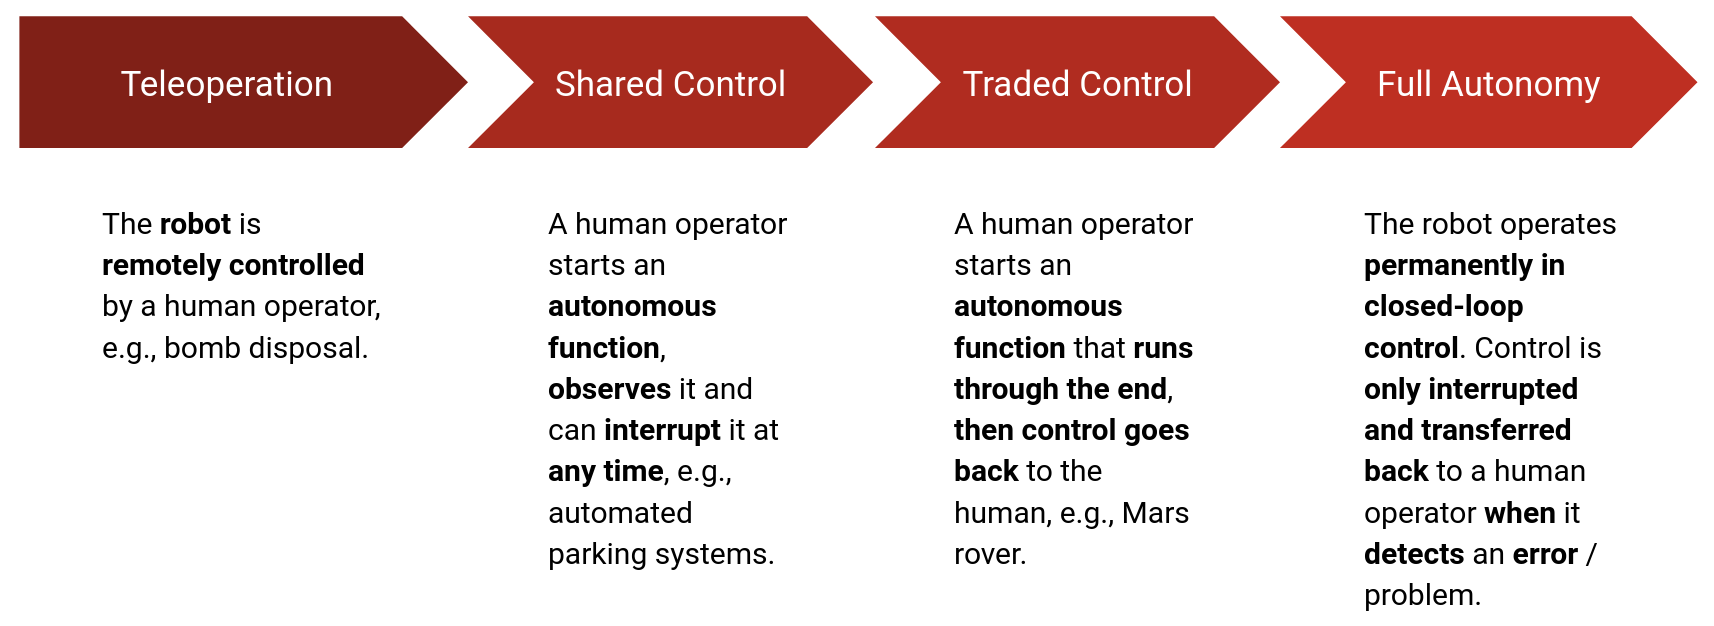
\includegraphics[width=\textwidth]{pics/autonomy_spectrum.png}
    \caption{\textsc{Autonomy Spectrum}}
    \label{fig:autonomy_spectrum}
\end{figure}
Accordingly, autonomy does not necessarily mean that there is no connection to a human operator at all.
The concept of traded control is particularly relevant for robotics in space applications, e.g. satellites or planetary rovers.
The idea is that the robotic system operates autonomously in principle, performing all the repetitive routine tasks, but the human operator can take over in certain situations,
such as when the robot is in danger and human intervention is required, or when a task needs to be performed that for some reason is better suited for a human operator.
\cite{Kortenkamp:2009}
The plant monitoring robot considered in this work, however, can be classified as fully autonomous in the sense of figure \ref{fig:autonomy_spectrum}, 
i.e. during a long-term autonomy cycle as defined above, the robot should only come into contact with a human operator when it detects an error or a problematic situation
that prevents it from continuing its task.

\section{Scientific and Technological Background}
\label{sec:scientific_bg}

The robotic system under consideration is going to be the autonomous robotic experimentation platform (AROX) \cite{Kisliuk:2021} that is assumed to integrate 
all the essential software and hardware required for the task at hand, i.e. processing a given plan (e.g. human provided) that causes the robot to autonomously
drive to specified locations and record scans. In addition to the actual physically available AROX, the system has been modeled in the unified robot description 
format (URDF) and can be used in a simulation. As starting point serves a physics simulation in Gazebo\footnote{Open-source 3D robotics simulator} that 
has been created within the research project PORTAL \cite{portal} and will be adapted and extended as part of this work. 
The simulation includes the AROX model, which is able to navigate autonomously to certain coordinates, as well as a 2.5D 
reflection of a test field and some abstract crops as objects of interest. Initially, the simulation works under the assumption that the robot is able to charge its 
battery as soon as it is located at certain coordinates as a simplification of the container infrastructure.
In order to determine the robot's route through the field as well as the whole scanning processes, a plan is needed, i.e. when to drive to and process which parcel of the field. 
For the basic prototypical system, it is simply assumed that the plans are generated by human operators. Hence, a plan is going to be a CSV file of actions.
Plan generation and format are described in detail in section \ref{sec:plan_generation}, but in general plans will focus on two types of actions.
The first type is \textsc{drive\_to(x, y)}, which causes the robot to drive to the specified coordinates (if possible), an action the employed robotic system 
AROX is capable of. The second type of action is \textsc{scan}, which initiates a scanning procedure at the robot's current position.
In practice, the real robot is equipped with a 3D-Lidar sensor that is going to be used to scan the field parcels with the aim of detecting features of the plants. 
To simulate the scanning procedure, some kind of dummy node is required that allows to scan on command, i.e. to simulate scanning, since we are not actually interested
in any scanning data. Thus, the second type of action will initiate a scanning procedure of the 3D-Lidar sensor or an execution of a dummy node, respectively.
There are other actions, but these two are the very specific ones relevant to the scenario under consideration; the details are described in section \ref{sec:plan_generation}.\newline
Kunze et al. point out that many challenges remain to be overcome with respect to the reliable deployment of long-term autonomous robots in real-world environments.
Particularly relevant to this work are the natural challenge of system integration, i.e. integrating numerous methods and technologies into a comprehensive solution 
for long-term autonomy, as well as the design of ``human-in-the-loop'' systems capable of utilizing the help of human operators in unexpected problematic situations. \cite{Kunze:2018}

\pagebreak

\section{Challenges}
\label{sec:challenges_for_lta}

Having clarified what long-term autonomy (LTA) means for this work, we now turn to potential problems that stand in its way.
There are numerous potential hinderances for long-term autonomous systems that can cause failure and prevent the system from continuing its task.
Without claiming to be exhaustive, the following is a list of potential problems in an agricultural field monitoring context that, from a practical perspective,
can prevent the smooth functioning of long-term autonomous systems and are thus worthy of investigation:
\begin{itemize}
    \item \textbf{power management} (battery failure / unexpected low battery)
    \item \textbf{charging failure} (unsuccessful docking / no charging)
    \item \textbf{drastic weather change} (e.g. storm, fog, extreme sunshine, heavy rain, extreme cold)
    \item \textbf{certain dynamics} (e.g. day / night)
    \item \textbf{sensor (perception) failure}
    \item \textbf{data management} (e.g. full memory, sensor data processing failure)
    \item \textbf{lost connection} (WiFi, RTK, UWB, LTE)
    \item \textbf{obstacles blocking planned path} (static / dynamic)
    \item \textbf{robot gets stuck} (e.g. spinning wheels)
    \item \textbf{robot falls over}
    \item \textbf{navigation failure} (\code{move\_base\_flex} / \code{pdc})
    \item \textbf{sustained recovery}, i.e. no return to \code{NORMAL\_OPERATION}
    \item \textbf{incorrect / inaccurate localization} (GPS, IMU, odometry)
    \item \textbf{mapping error} (e.g. incorrect costmap entries)
    \item \textbf{plan deployment failure}, i.e. robot remains in \code{IDLE}
\end{itemize}
For each potential problem identified, its relevance, i.e. the reasons why it might be problematic, and its consequences are briefly explained below.
The idea is to have monitoring nodes that look for the specific types of issues and report them via the \code{MonitorState}s topics,
which triggers a transition to \code{CONTINGENCY} or \code{CATASTROPHE}. Depending on the type of problem, information on the required method of resolution 
is transmitted via the published message. Therefore, the overall goal is to have a resolver node for each of the potential failures that is executed in \code{CONTINGENCY} 
or \code{CATASTROPHE} based on the failure case at hand. The entire process is essentially the same for all potential LTA problems - fault simulation, monitoring, 
and subsequent remediation.

\pagebreak

\noindent
\textbf{Power Management}\newline

\noindent
A natural requirement for LTA systems is some kind of energy management. The system is expected to operate autonomously for extended periods of time, which of course 
assumes a power supply. However, the energy management estimated at planning time may not work correctly or as expected at execution time, e.g. the battery could be 
low before the planned time. Or worse, there could be a complete battery failure. It would certainly be useful to enable the system to handle such issues, at least to 
some degree. A watchdog module that monitors the battery state and acts as a fail-safe, such as the one described in section \ref{sec:battery_monitoring}, could be 
integrated to address power management issues and improve the robot's survivability.\newline

\noindent
\textbf{Charging Failure}\newline

\noindent
Another category of potential LTA problems related to the system's power supply is charging failures. Several things can go wrong during a charging process. 
Leaving aside the simplistic assumption of charging upon arrival at specific coordinates and considering the actual charging process 
in practice with the AROX system, it must dock with an inductive charging station in a mobile container at the field site.
Accordingly, docking to the charging station may fail or the charging process itself may not start after docking.
Both cases should be detected by the robot so that an appropriate reaction can be initiated, e.g. informing the human operator.\newline

\noindent
\textbf{Drastic Weather Change}\newline

\noindent
Since the system is designed for moderate weather conditions, drastic weather changes can also play a role.
If the weather changes too drastically, it can be problematic for various aspects of the system.
If it is stormy, for example, this can be delicate for the sensor recordings, but also for the robot platform itself, as it could fall over.
The quality of the sensor images can also be affected by fog or extreme sunlight (illumination).
In addition, heavy rain should also be avoided. Finally, extreme cold could be a major problem for the system's battery.
In general, it would be good to identify such extreme weather conditions that could affect the functioning of the system in order to respond accordingly.\newline

\noindent
\textbf{Certain Dynamics}\newline

\noindent
Similar to weather changes, there are other dynamics such as the natural transition from day to night. For sunlight-dependent sensors such as cameras, 
the robot should take twilight into account and plan its operations accordingly to be back in the shelter, i.e. the mobile container, by dark.\newline

\noindent
\textbf{Sensor (Perception) Failure}\newline

\noindent
Hardware issues are a very general problem class and could relate to almost arbitrary many kinds of issues.
Since the correct functioning of the 3D-Lidar sensor is crucial for the long-term monitoring scenario,
the main focus will be on detecting hardware faults of this type. Sensor failures are, of course, a failure class in which the robot can do little except 
attempt to restart the corresponding sensor, and therefore rarely has any choice but to call the human operator for assistance. 
Nevertheless, it is important to identify such a malfunction as soon as possible, communicate the problem and avoid a lot of useless work and wasted operating time.
A fairly trivial approach to detecting sensor failures would be to simply check whether messages are still arriving on the corresponding ROS topic.
While trivial, it is not yet available and is critical for reasonable long-term autonomy. Moreover, it is quite easy to evaluate such a failure case,
as it can be easily simulated by stopping to publish laser scans in the dummy scanner node. In such a case, a monitoring procedure should be able to detect this,
switch to \code{CONTINGENCY} mode and call for help, for example. The idea is then to demonstrate that in the prototypical scenario, the plan will no longer 
execute correctly when these errors occur, and then after monitoring is started, the problem is detected, the operator is informed, the problem is resolved, 
and plan execution can continue. Such a simulated sensor failure can also be triggered by publishing on some topic.\newline

\noindent
\textbf{Data Management}\newline

\noindent
Since the overall objective of the robot's missions is to acquire data, the appropriate management of this data is of relevance.
If, for example, the robot is no longer able to save further scans due to a full memory, it should recognize and communicate this.
In addition, there may be disturbances in the processing of the sensor data, so that the robot is no longer able to process and save the recordings correctly.
It would be valuable to identify such problems as soon as possible to avoid redundant missions.\newline

\noindent
\textbf{Lost Connection}\newline

\noindent
For the robot to work as expected, it must maintain connections to various services. Accordingly, an interruption of one of these connections should be detected immediately.
A real time communication channel (e.g. WiFi) is required to connect the RTK base station, i.e. the mobile container, and the RTK rover, i.e. the robot, in order to
transmit the correction signals for high-precision positioning. Furthermore, it is crucial that both the robot and the base station receive their own GNSS signals,
i.e. are connected to the GNSS service. In addition, the RTK-GNSS data is used for scan registration. Finally, the recorded scans are transmitted via WiFi or LTE 
to the base station or external servers for further processing.\newline

\noindent
\textbf{Obstacles Blocking the Planned Path}\newline

\noindent
A relatively common problem for the long-term autonomy of a mobile robot is obstacles blocking the planned path.
A rough distinction can be made between static obstacles such as a trailer and dynamic obstacles such as animals or people.
The used navigation framework \code{move\_base\_flex} can already detect obstacles and initiate a recovery behavior if the planned path is not traversable.
However, it would be good to refine the default recovery behaviors and adapt them to the scenario at hand. Recovery behaviors should naturally vary between
static and dynamic obstacles. A dynamic obstacle like a person or an animal will in most cases simply walk through the scene and disappear a moment later,
so waiting for a moment can already be a very reasonable and sufficient recovery behavior. Static obstacles, on the other hand, may be present for longer 
periods of time, requiring more sophisticated recovery behaviors.\newline

\noindent
\textbf{Robot Gets Stuck}\newline

\noindent
(e.g. spinning wheels due to a muddy path)\newline
TBD...\newline

\noindent
\textbf{Robot Falls Over}\newline

\noindent
TBD--\newline

\noindent
\textbf{Navigation Failure}\newline

\noindent
Another issue that was already present in experiments during this work.
The global planner provides a path that tries to drive around a field although there is no way.
Also in "Don’t Make the Same Mistakes Again and Again: Learning Local Recovery Policies for Navigation from Human Demonstrations"\newline
TODO: REFINE:::: \newline
e.g. global plan not feasible\

\noindent
\textbf{Sustained Recovery}\newline

\noindent
i.e. not getting back to normal operation\newline

\noindent
\textbf{Incorrect or Inaccurate Localization}\newline

\noindent
It is obvious that it is a problem when the robot is not able to localize itself correctly in its environment.
In this case, it is a matter of localization within a global reference system, i.e. determining the pose (position and orientation) within a given map of the environment.
If the localization is no longer accurate, e.g. because the robot has been moved to a different position in the map, it must detect this in order to
trigger relocalization. In the case of such a localization error, the \textit{kidnapped robot problem} arises, because although no one has 
physically moved the robot from its position, it is the same from the robot's perspective. \cite{Hertzberg:2012}
The relevance here can easily be argued based on practical experience, as this issue has already caused a lot of trouble in practice with the AROX system during 
the work for the PORTAL project. In these situations, a major problem for localization was rotating the robot on the spot.
The problems encountered consisted mostly of an incorrect orientation of the robot and rather rarely of an actual incorrect position.
If the orientation is incorrect, the sensor records will also be incorrectly aligned, which is a major problem for the scenario under consideration.
It would be very valuable to develop a monitoring  approach that is capable of realizing situations in which the localization is no longer accurate, as there is a
simple workaround that alleviates the problem in practice in many cases: Just driving the robot a few meters back and forth to recalibrate the localization 
using different GPS positions. Of course, it can also be a problem for localization if the GPS signal itself is inaccurate or non-existent, but that is another topic.\newline
TODO: lack of GPS signal is going to be discussed here...\newline

\noindent
\textbf{Mapping Issues}\newline

\noindent
incorrect costmap entries due to incorrectly perceived 'virtual objects' (e.g. detect ground as obstacle)\newline

\noindent
\textbf{Plan Deployment Failure}\newline

\noindent
i.e. robot keeps in \code{IDLE} state too long, because no plan arrives -> should be recognized\newline

TODO\newline

\noindent
\textbf{Communication with a Human Operator}\newline

\noindent
TODO: Not yet sure where to put this..\newline
Communication with a human operator, i.e. notifying a human operator that a problem has occurred that requires human intervention,
is implemented as the ROS topic \code{\/request\_help}. Once the problem has been solved by the human operator, the control can be returned
to the autonomous mobile robot via the \code{\/problem\_solved} topic.\newline

The idea is to tackle a subset of this potentially extended list of issues that is realistically solvable in the scope of the work.
Generally, the potential barriers for long-term autonomy can be classified into three categories of increasing impact on the system:
\begin{enumerate}
    \item The robot recognizes a problem and is able to solve it by itself.
    \item The robot recognizes a problem, is unable to solve it, and calls a human operator for help.
    \item The robot has a malfunction / problem, but does not recognize it and is therefore unable to solve or communicate it.
\end{enumerate}
In the baseline scenario, i.e. a running prototype of an integrated solution, each potential issue in the above list will be classified as type $(3)$.
Part of the goal of this work is to shift the problems of the selected subset to another category, i.e. to solve them completely, 
or at least to enable the robot to recognize them with execution monitoring approaches and request help.
However, it is also part of the truth that not all possible external influences are solvable, i.e. a robot will not be able to solve all
conceivable problems itself. Long-term autonomy has its limits, and there are simply unpredictable situations that a mobile robot cannot be expected to handle,
e.g. if its battery bursts into flames, or it is knocked over by something. In such a case, the only way to do damage control is to try to shut down the 
robot in a controlled manner (e.g. with data backup) and, if possible, communicate the problem.
Of course, one could assign probabilities to specific incidents, which vary depending on the information available. 
For example, if the robot detects that the battery is showing unusual discharge behavior, such information could be taken into account and 
reported to the operator. Nevertheless, it's not feasible to cover everything that can happen, and long-term autonomy is subject to certain limits.

\chapter{Plan Execution and Monitoring}

A key aspect of handling some of the potential issues introduced in section \ref{sec:challenges_for_lta} is going to be that the robot will not be able to
complete its missions without preempting the plan execution from time to time. Either due to insufficient battery capacity or other unmanageable conditions such as 
drastic weather changes that force the robot to interrupt its task. Although the overall route may always be the same for the same field, there are certain stopping
conditions that cause the robot to interrupt its active scanning tour and possibly drive back to its base, i.e. the mobile container.
There are generally two relevant perspectives. First, such stops have to be considered at planning time by acknowledging charge stops as crucial part of the plan.
Of course, this is only covering plannable stops such as expected battery consumption and is not able to deal with unplanned situations.
Therefore, a second perspective comes into play, that will be particularly relevant in this work - the execution time.
Just as important as the planning itself is the execution of the generated plan as well as monitoring the execution.
The idea is that the robot executes a given plan and is somehow capable of realizing that it has to interrupt the execution due to some unexpected condition.
In such a case, the robot needs to be able to save the current state of the plan execution and continue precisely with this state after the reason 
for the interruption has been resolved. Consequently, the robot has to be prepared to pause and resume the execution of a given plan, which is far from 
trivial, since the original plan may no longer be applicable for various reasons.

\section{Execution Monitoring State Machine Architecture}
\label{sec:execution_monitoring_smach_architecture}

Plan execution as well as robot operation monitoring are modeled as a high-level hierarchically structured state machine, whose architecture is shown
in figure \ref{fig:high_level_smach}. The architecture is implemented using the SMACH\footnote{ROS-independent Python library to build hierarchical state machines \cite{smach}} 
library.
\begin{figure}[H]
    \centering
    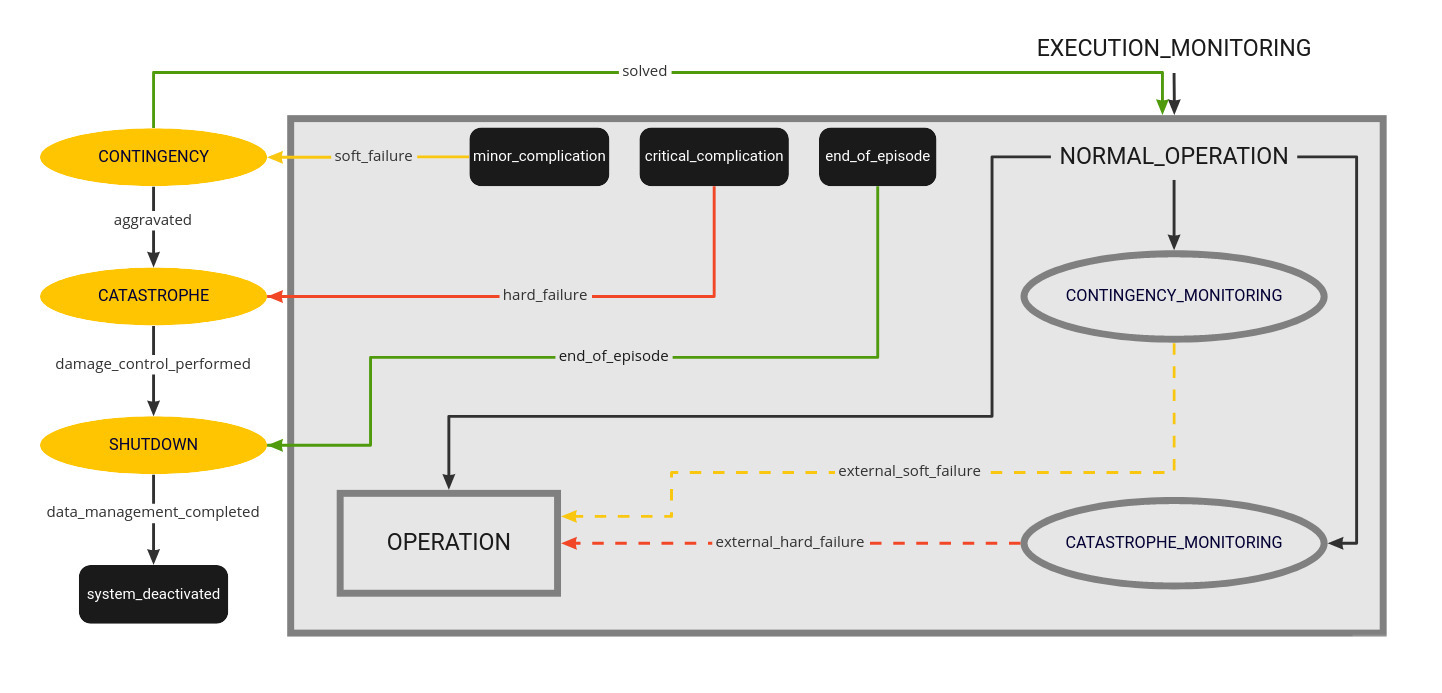
\includegraphics[width=\textwidth]{pics/SMACH_high_level_pretty.jpg}
    \caption{\textsc{Architecture of the Hierarchical State Machine (High-Level)}}
    \label{fig:high_level_smach}
\end{figure}
\noindent
As depicted in figure \ref{fig:high_level_smach}, the robot starts in the state \code{NORMAL\_OPERATION} in the high-level hierarchical state machine \code{EXECUTION\_MONITORING}.
\code{NORMAL\_OPERATION} is represented by an embedded state machine named \code{OPERATION}, visualized in figure \ref{fig:low_level_smach}, as well as the two
parallel running execution monitoring states (cf. ROS \code{MonitorState} \cite{monitor_state}) \code{CONTINGENCY\_MONITORING} and \code{CATASTROPHE\_MONITORING}, 
implemented as a concurrence container (cf. SMACH \code{Concurrence} \cite{concurrence_container}).
These parallel running states are used to monitor the robot's operation and to interrupt it when a problematic situation requiring special treatment is detected
(see the dashed arrows in figure \ref{fig:high_level_smach}).
Although a monitoring solution could in principle also be implemented sequentially, it seems more natural to choose a parallel approach, since a sequential option
would have the disadvantage that no monitoring takes place while a task / algorithm is being executed, but only afterwards.
It is desirable to be able to intervene at any time during the execution of a task when a monitoring procedure running in parallel is triggered and causes a change of state.
During the state \code{OPERATION}, i.e. in the nested state machine visualized in figure \ref{fig:low_level_smach}, the robot can be either in the state \code{IDLE}, 
in which it is waiting for a plan, or in \code{EXECUTE\_PLAN}, in which it is executing a given plan. The embedded state machine \code{OPERATION} has 
four possible outcomes - \code{end\_of\_episode}, \code{minor\_complication}, \code{critical\_complication}, and \code{preempted}. 
It starts in the \code{IDLE} state and remains there as long as no plan is provided via a ROS service.
There are two common options for the robot to leave the state. The first is via a message on a ROS topic indicating that the end of the current long-term episode
has been reached, resulting in an overall outcome of \code{end\_of\_episode} for \code{NORMAL\_OPERATION}. The second is to receive a plan that results in a state
transition to \code{EXECUTE\_PLAN}. Additionally, the external parallel running monitoring states \code{CONTINGENCY\_MONITORING} and \code{CATASTROPHE\_MONITORING}
are capable of interrupting the \code{IDLE} state at any time (cf. state preemption \cite{state_preemption}) due to external problems leading to the outcome \code{preempted}.
In \code{EXECUTE\_PLAN}, there are five possible outcomes, two of which result in state transitions and three of which cause \code{OPERATION} 
to return to the parent state machine. The first possible outcome is \code{action\_completed}, which indicates that an action of the currently processed plan was 
completed successfully and causes the same state (\code{EXECUTE\_PLAN}) to be executed again with the reduced plan, i.e. the rest of the plan is executed.
The next possible outcome is \code{plan\_completed}, which means that the entire plan has been successfully processed and causes a transition back to the \code{IDLE} state.
These were the possible outcomes that cause a transition to another state. Now there are the three remaining outcomes that cause a return to the parent state machine. 
First, \code{soft\_failure}, which means that something went wrong, e.g. an action was not performed successfully, but the robot should be able to handle the problem. 
Second, there is the potential outcome \code{hard\_failure}, which represents situations where the robot is unable to solve the problem itself.
Finally, the last potential outcome is again \code{preempted} based on some external issue detected by \code{CONTINGENCY\_MONITORING} or \code{CATASTROPHE\_MONITORING}.
\begin{figure}[H]
    \centering
    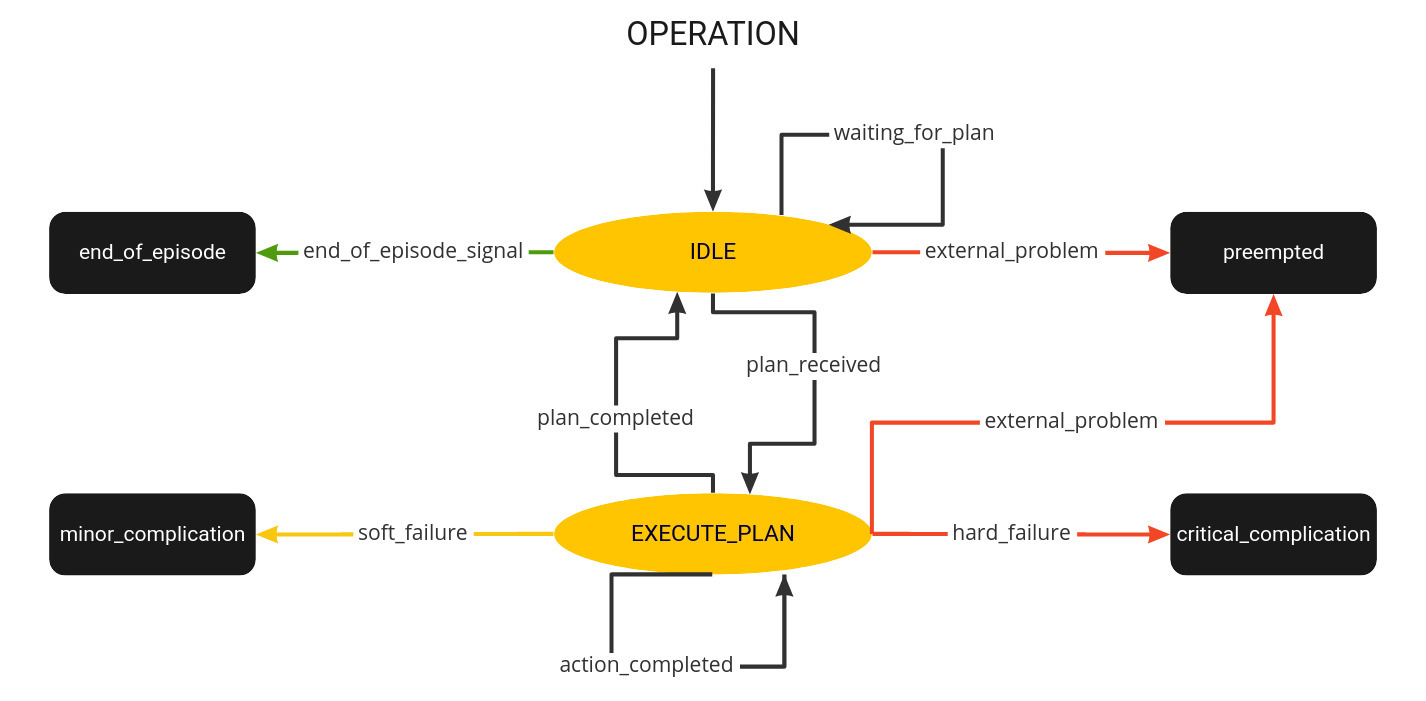
\includegraphics[width=\textwidth]{pics/SMACH_low_level_pretty.jpg}
    \caption{\textsc{Architecture of the Embedded State Machine (Low-Level)}}
    \label{fig:low_level_smach}
\end{figure}
\noindent
Now that the control flow of \code{NORMAL\_OPERATION} and, in particular, \code{OPERATION} has been clarified, we return to the parent state machine shown 
in figure \ref{fig:high_level_smach}.
As mentioned, when \code{NORMAL\_OPERATION} returns \code{end\_of\_episode}, the parent state machine transitions to the \code{SHUTDOWN} state and the 
robot's work for that long-term episode is complete, which means that the robot performs data management and then the system is deactivated.
Essentially, in a long-term episode in the considered scenario, the robot should stay in \code{NORMAL\_OPERATION} as 
long as the episode is running or an error / problem has occurred, either an error that it is able to deal with itself or even a more severe problem that requires the 
intervention of a human operator. Accordingly, if \code{NORMAL\_OPERATION}, i.e. the embedded state machine together with the parallel running monitoring states has the outcome 
\code{minor\_complication}, the robot enters the state \code{CONTINGENCY}, which means that it has detected a soft failure, e.g. a sensor failure, but its ability to act
is preserved, it is for example able to drive back to the base in safety mode. However, if \code{NORMAL\_OPERATION} returns \code{critical\_complication}, there is a hard 
failure that is unsolvable for the robot, perhaps even for the operator, and the robot transitions to \code{CATASTROPHE}. If it is still possible, the robot saves the current 
state of the plan execution, sends an emergency signal, e.g. communicates the problem to the operator, and shuts down, i.e. transitions to \code{SHUTDOWN}.
There are, of course, situations in which the robot can no longer do anything, such as when the battery is completely discharged.
In principle, such cases also fall under the category of catastrophe, but since monitoring then no longer works, there is nothing left to do there.
Besides, there are two more transitions depicted in figure \ref{fig:high_level_smach}: From \code{CONTINGENCY} back to \code{NORMAL\_OPERATION}, after a minor problem is resolved by the robot, it can continue
its normal operation. Additionally, it is possible that something goes wrong during \code{CONTINGENCY} or that the problem actually cannot be solved by the robot,
such that it transitions to \code{CATASTROPHE}.\newline
To be clear, \code{NORMAL\_OPERATION} can manage problems in two ways.
First, a problem may occur during plan execution in the child state machine, in such a case \code{OPERATION} returns \code{critical\_complication} or 
\code{minor\_complication} to the parent state machine based on the problem severity and a corresponding state transition takes place.
In addition, there are the described parallel monitoring states, which are responsible for problems that are not directly related to plan execution, but are of a more general nature.
If these detect a problem, they are able to interrupt \code{OPERATION} and also return \code{critical\_complication} or \code{minor\_complication} to the parent state machine
\code{EXECUTION\_MONITORING}.\newline
The general difference between the \code{CONTINGENCY} and \code{CATASTROPHE} states is the robot's ability to act. 
In a catastrophe case, it is no longer really capable of acting in the sense of driving back to its base, managing the problem itself, etc. 
An example for a catastrophic case would be that the robot falls over. It is then unable to recover, but it is of course still able to communicate the problem
and save the state, in full possession of its ``mental'' powers, so to speak. Whereas a lightning strike, as an extreme example, could cause the robot to have a 
complete breakdown and nothing to work at all. The boundaries there are not quite sharp, there are many edge cases.
The following somewhat more mundane example, considering the robot's battery, will illustrate the concepts.
In \code{NORMAL\_OPERATION}, the battery discharges according to the plan. There may be some fluctuations due to temperature, for example, but it works roughly as expected.
It would transition to the state \code{CONTINGENCY} when it detects that the battery is already too low to complete the plan, but it is still able to recover,
i.e. drive back to its base, recharge, and continue the plan execution. However, it would proceed to \code{CATASTROPHE} if it detects that the battery is so low
that it can already tell that it is not possible to reach the base and recharge. It is then still able to communicate the problem and save the state, but it is not able
to recover. The extreme case, where nothing can be done, would be that the battery suddenly just breaks.

\pagebreak

\section{Plan Generation and Format}
\label{sec:plan_generation}

Long-term autonomous robot operation commonly includes following some sort of plan. However, since the actual planning is not part of this work, it is assumed that
plans are provided and usable, e.g. handcrafted by a human operator or generated by a planner from the literature.
For the purpose of parsing such plans and making them retrievable via a service call, a ROS node was developed.
In order for the node to parse the plans, they must be formulated in the following CSV format.
There are four available actions - \code{drive\_to}, \code{return\_to\_base}, \code{charge}, and \code{scan}.
Each line in the CSV file represents one action of the plan. The actions \code{return\_to\_base}, \code{charge} and \code{scan} have no parameters,
but \code{drive\_to} needs the additional arguments \code{latitude}, \code{longitude} and \code{orientation} of the target pose.
An example for a simple plan is shown in figure \ref{fig:plan_example}. 
When the robot executes this plan, it drives to the four specified locations in sequence and records scans.
Afterwards, it returns to the base and recharges its battery.
\begin{figure}[H]
    \centering
    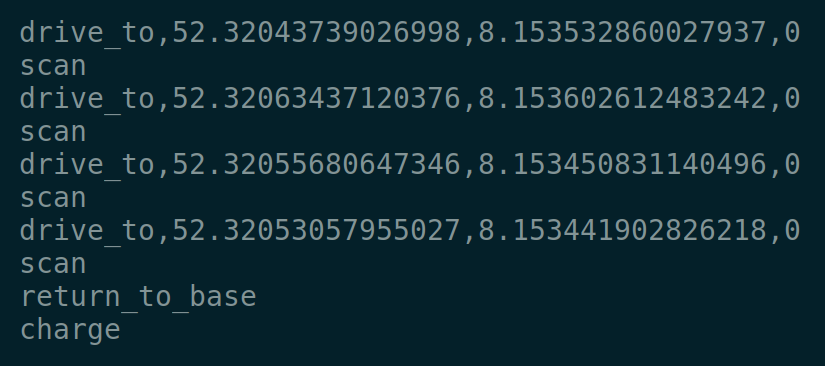
\includegraphics[width=0.5\textwidth]{pics/plan_example.png}
    \caption{\textsc{Sample Plan}}
    \label{fig:plan_example}
\end{figure}
\noindent

\section{Interrupt and Resume Normal Operation}

In order to handle unexpected problematic situations, the robot must be able to stop and resume its normal operation in general
and plan execution in particular, i.e. to save the current state of the plan execution and resume exactly that state after the reason
for the interruption has been resolved. The idea is that whenever the monitoring procedures \code{CONTINGENCY\_MONITORING} and \code{CATASTROPHE\_MONITORING} 
introduced in section \ref{sec:execution_monitoring_smach_architecture}, or the plan execution itself, detect a problem, they should trigger such an interruption.
As seen in the last section, there are two states in \code{OPERATION} that the robot can be in during a long-term episode without any problems
- \code{IDLE} or \code{EXECUTE\_PLAN}. In the \code{IDLE} state, where it waits for the plan generator described in section \ref{sec:plan_generation} to provide a plan,
it is straightforward, the normal operation is interrupted, the high-level state machine transitions to \code{CONTINGENCY} or \code{CATASTROPHE} depending
on the severity of the problem, and then, i.e. when the minor problem is resolved, it transitions back to \code{IDLE} or, in the case of \code{CATASTROPHE},
it shuts down. The more interesting case, of course, is such an interruption of normal operation when the robot is in the low-level state \code{EXECUTE\_PLAN}.
During the \code{EXECUTE\_PLAN} state, the currently executed plan is always stored in the \code{userdata} field of the state.
SMACH states always provide so-called \code{userdata} fields, which are essentially the input and output data of a SMACH state.
Initially, when \code{IDLE} receives a plan from the plan generator, it passes it as \code{userdata} to the \code{EXECUTE\_PLAN} state.
Then, whenever \code{EXECUTE\_PLAN} successfully completes an action of the plan, the reduced plan is passed to the next iteration of the same state.
Therefore, based on this architecture, the current state of the plan execution is always stored in the \code{userdata} of the SMACH.
Of course, when the robot transitions back to \code{NORMAL\_OPERATION} after solving a contingency, it starts again in \code{IDLE}, which is why \code{IDLE} 
always looks for existing unfinished plans in the \code{userdata} first. If there is one, it does not prompt the plan generator for a new plan, but continues the previously 
preempted plan. The catastrophe case works analogously to the \code{IDLE} state.

\chapter{Integrated Solutions}

In general, an integrative work benefits from many integrated solutions. Nevertheless, it should be viable in the scope of the work and robust.
Essentially, there is a tradeoff between integrating as much as possible, thereby increasing the functionality, and staying feasible and realistic.
The following subsections present exemplary approaches that may be integrated. The list could be expanded as needed during the course of the work.

\section{Battery Monitoring}
\label{sec:battery_monitoring}

One solution that could be worth integrating is a watchdog module that observes the battery state and acts as a fail-safe. In principle, the charge stops should
be part of the plan, i.e. be considered at planning time. Thus, there has to be resource planning for the missions that includes to be back at the base station before
the robot runs out of battery. However, if it fails, there could be a monitoring process at execution time that is able to react to wrong plans, i.e. the battery is
low before expected and the robot has to return to its base. The module essentially checks the distance from the robot's current position to the base station, 
the expected battery consumption to get there, and the remaining battery charge. In summary, the module is running at execution time, it does not schedule the 
charge stops in advance, but only responds to failure cases where the robot needs to preempt the plan execution, return to its base and recharge.
Such a battery watchdog is an example for monitoring tools relevant for addressing the challenges introduced in section \ref{sec:challenges_for_lta}.

\section{Autonomous Energy Supply}

A fundamental step towards long-term autonomy of a mobile robot is to ensure its power supply.
For this purpose, there is an inductive charging station located in a mobile container on the field site.
Thus, the power supply could be realized by integrating an autonomous docking / undocking solution that enables the robot to detect
the container in a laser scan of its nearby surroundings, drive into it and dock to the inductive charging station.
This docking solution could be used for both planned charge stops as well as unexpected but necessary stops detected by monitoring processes such
as the one described in section \ref{sec:battery_monitoring}.

% DON'T set \bibliographystyle here -- use the documentclass option instead
\bibliography{papers}

\closing %%%%%%%%%%%%%%%%%%%%%%%%%%%%%%

\end{document}
